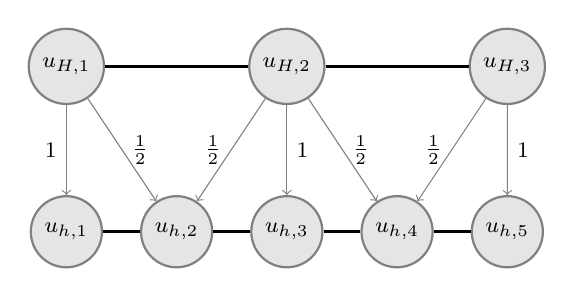
\begin{tikzpicture}[node/.style={circle,draw=black!50,fill=black!10,thick,font=\footnotesize},scale=0.7,
arrownote/.style={black,font=\footnotesize}]


\node (u1) at (0,3) [node] {$u_{H,1}$};
\node (u2) at (4,3) [node] {$u_{H,2}$};
\node (u3) at (8,3) [node] {$u_{H,3}$};


\node (u5) at (0,0) [node] {$u_{h,1}$};
\node (u6) at (2,0) [node] {$u_{h,2}$};
\node (u7) at (4,0) [node] {$u_{h,3}$};
\node (u8) at (6,0) [node] {$u_{h,4}$};
\node (u9) at (8,0) [node] {$u_{h,5}$};

\draw [very thick] (u1) -- (u2) --(u3);
\draw [very thick] (u5) --(u6) --(u7) --(u8) --(u9);

\draw [->,black!50] (u1) to node [arrownote,left] {$1$}  (u5) ;
\draw [->,black!50] (u1) to node [arrownote,right] {$\frac{1}{2}$} (u6) ;

\draw [->,black!50] (u2) to node [arrownote,left] {$\frac{1}{2}$} (u6) ;
\draw [->,black!50] (u2) to node [arrownote,right] {$1$} (u7) ;
\draw [->,black!50] (u2) to node [arrownote,right] {$\frac{1}{2}$} (u8) ;

\draw [->,black!50] (u3) to node [arrownote,left] {$\frac{1}{2}$} (u8) ;
\draw [->,black!50] (u3) to node [arrownote,right] {$1$} (u9) ;

\end{tikzpicture}